\subsection*{Teil B: Negative Zahlen (20 Minuten)}

\begin{enumerate}[resume, label=\arabic*.]
    \item \textbf{Trage auf dem Zahlenstrahl ein:}

    Die Punkte: $-2,5$ ; $1,5$ ; $-0,5$ ; $3$   

    \begin{center}
        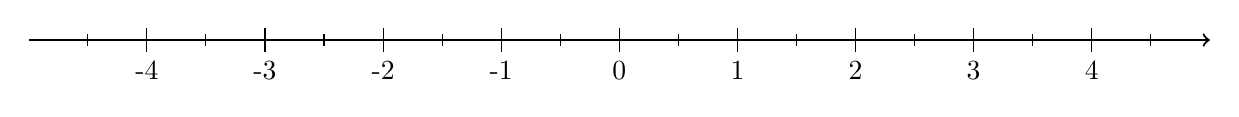
\begin{tikzpicture}[scale=1.5]
            \draw[thick,->] (-5,0) -- (5,0);
            \foreach \x in {-4,-3,-2,-1,0,1,2,3,4}
            \draw (\x,0.1) -- (\x,-0.1) node[below] {\x};
            \foreach \x in {-4.5,-3.5,-2.5,-1.5,-0.5,0.5,1.5,2.5,3.5,4.5}
            \draw (\x,0.05) -- (\x,-0.05);
        \end{tikzpicture}
    \end{center}

    \vspace{0.8cm}

    \item \textbf{Temperaturaufgaben:}
    \begin{enumerate}[label=\alph*)]
        \item Morgens sind es $-3°C$, mittags steigt die Temperatur um $7°C$. \\
        Wie warm ist es mittags?

        \vspace{0.3cm}
        Rechnung: $-3°C + 7°C$ = \underline{\hspace{3cm}}

        \vspace{0.3cm}
        Antwort: Mittags sind es \underline{\hspace{3cm}} Grad.

        \vspace{0.5cm}
        \item Abends sind es $2°C$, nachts fällt die Temperatur um $5°C$. \\
        Wie kalt ist es nachts?

        \vspace{0.3cm}
        Rechnung: $2°C - 5°C$ = \underline{\hspace{3cm}}

        \vspace{0.3cm}
        Antwort: Nachts sind es \underline{\hspace{3cm}} Grad.
    \end{enumerate}

    \vspace{0.8cm}

    \item \textbf{Vergleiche} (Setze $<$, $>$ oder $=$ ein):

    \vspace{0.3cm}
    \begin{tabular}{llll}
        a) $-3$ \underline{\hspace{1cm}} $-1$ & 
        b) $-5$ \underline{\hspace{1cm}} $0$ & 
        c) $2$ \underline{\hspace{1cm}} $-2$ & 
        d) $-4$ \underline{\hspace{1cm}} $-4$
    \end{tabular}

    \textit{Tipp: Die Zahl weiter rechts auf dem Zahlenstrahl ist größer!}
\end{enumerate}